\graphicspath{ {../images/} } 

In Tabelle \ref{table:1} vergleichen wir die Vor- und Nachteile der beiden Paradigmen Sprach und Aktion:
\begin{table}[h!]
\centering
  \begin{tabular}{||p{3cm}|p{5cm}|p{5cm}||} 
 \hline
 & Vorteile & Nachteile \\ [0.5ex] 
 \hline\hline
 Sprachparadigma & Leistungsfähig, flexibel, grosse Automationsmöglichkeit &
    Keine Signifier, Nur recall und keine recognition möglich \\ [1.5ex] 
    & & \\
 Aktionsparadigma & Feedback, Sichtbarkeit, Reversibleaktionen & Recognition nur
  möglich wenn ein standard Desgin umgesetzt wird, oft weniger
  Automationsmöglichkeiten \\
 \hline
\end{tabular}
\caption{Vergleich Sprach- und Aktionsparadigma}
\label{table:1}
\end{table}

Es gibt aber auch Beispiele welche sowohl eine Sprachparadigma sowie ein
Aktionsparadigma anbieten. Wir haben uns hier für das Webinterface von
DigitalOcean entschieden, welches die Möglichkeit bietet Server-Eintstellungen
sowohl über die Webseite, wie auch über einen Terminal-Zugriff (via Web)
durchzuführen:

\begin{figure}[h]
  \caption{Webinterfacezugriff auf Droplet/Server}
  \centering
  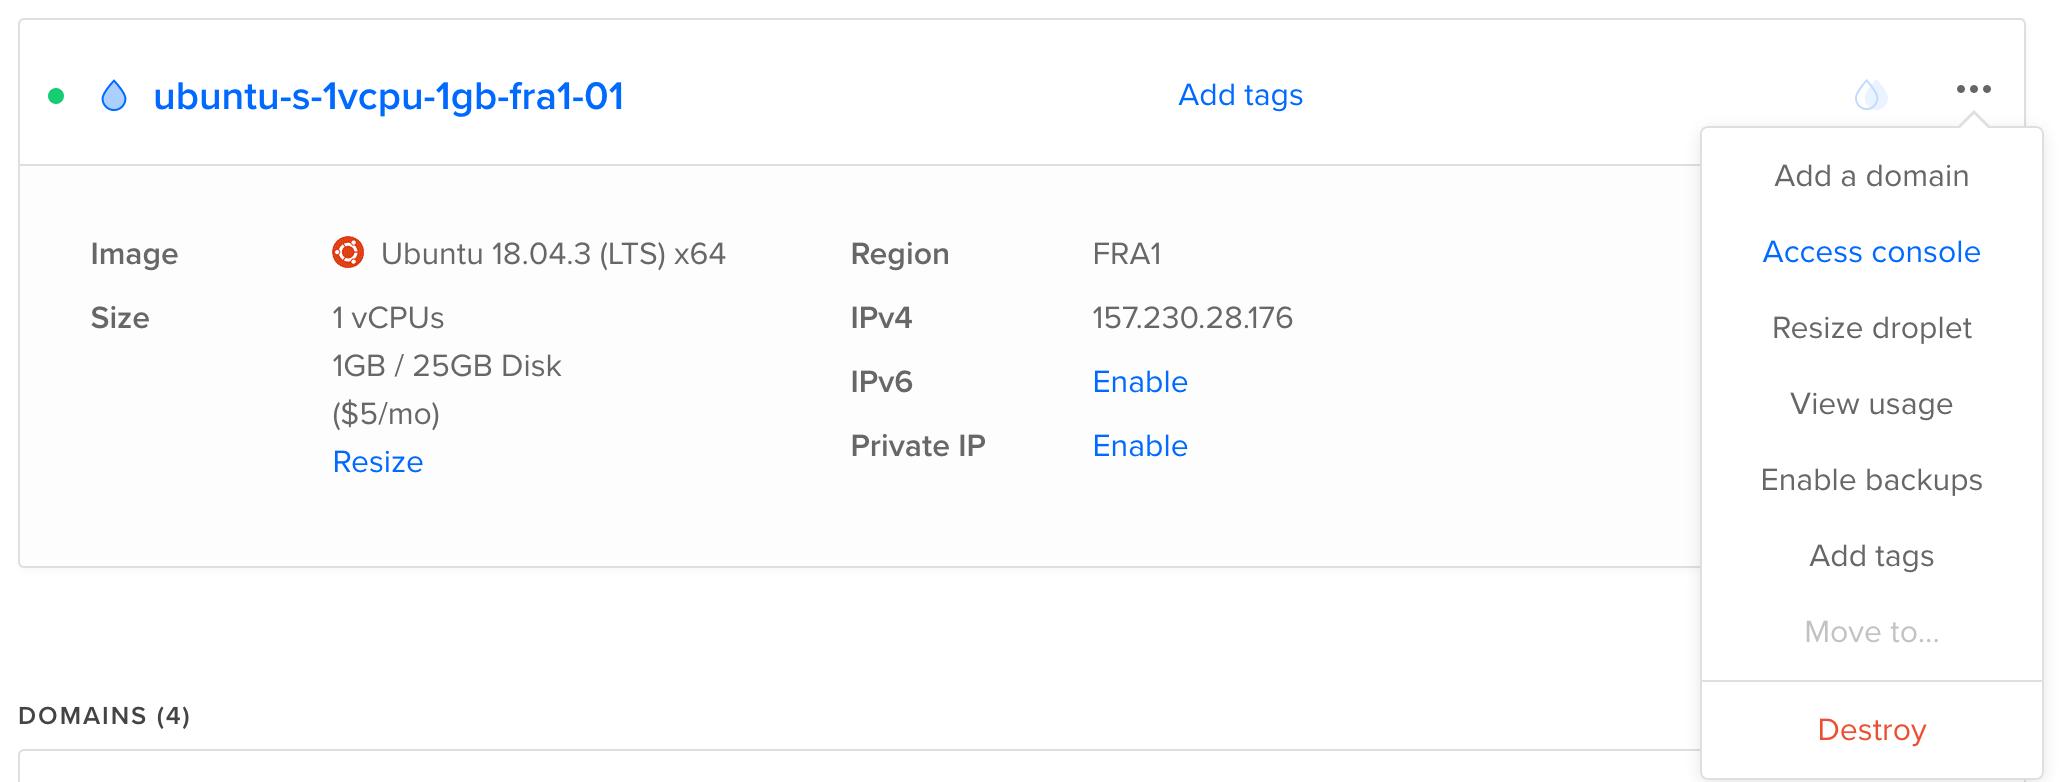
\includegraphics[width=0.7\textwidth]{digitalocean1}
\end{figure}


\begin{figure}[h]
  \caption{Terminalzugriff auf Droplet/Server}
  \centering
  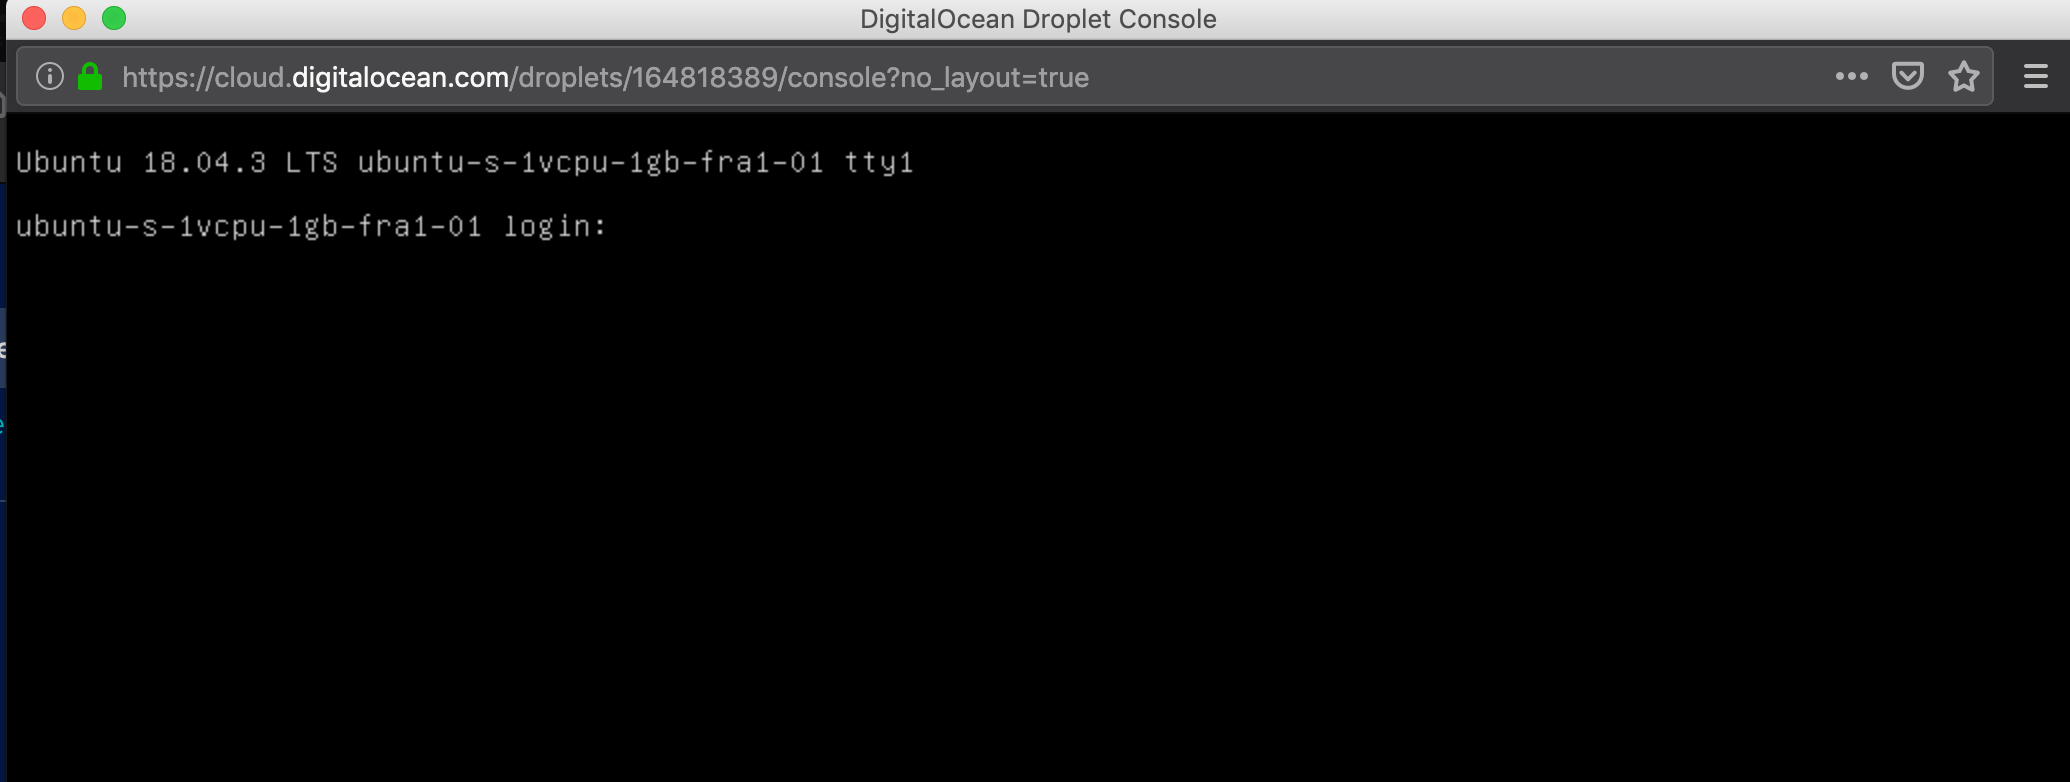
\includegraphics[width=0.7\textwidth]{digitalocean2}
\end{figure}
